\begin{figure}[h!]
\begin{center}
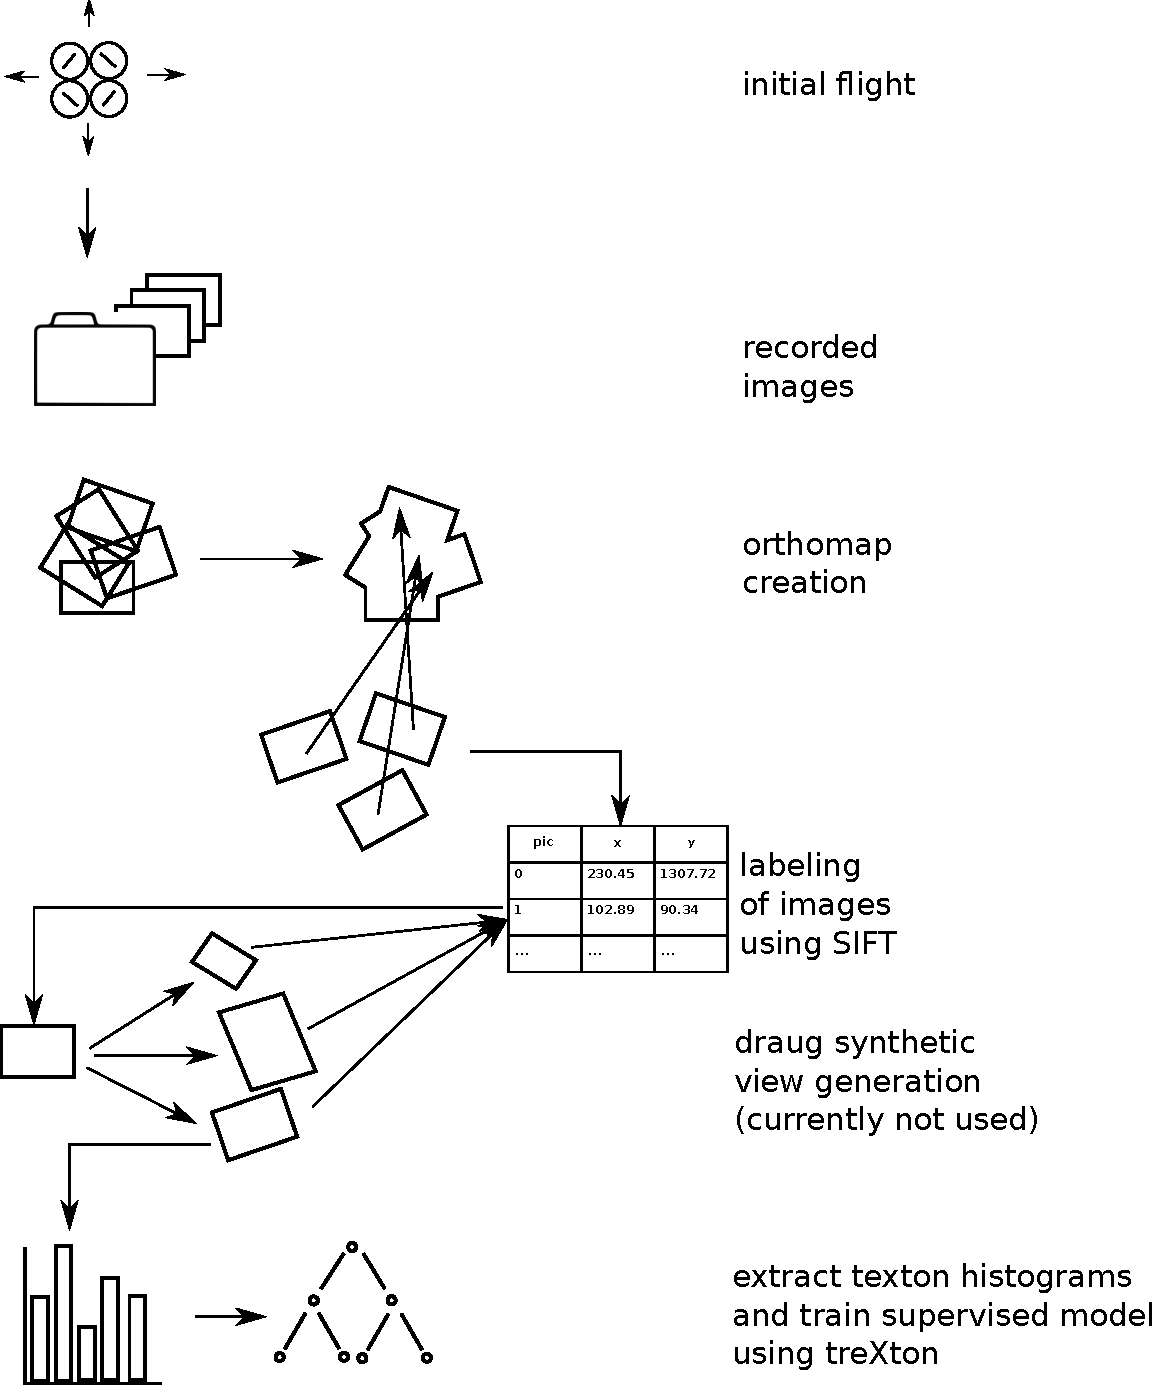
\includegraphics[width=0.7\columnwidth]{figures/overview}
\caption{{\label{fig:overview}
}}
\end{center}
\end{figure}

\section{Hardware and Software of the Platform}
\label{sec:hardware}

In a first setting, the commercially available Parrot AR.Drone2.0 was
equipped with an Odroid XU-4 single board computer, a Logitech 525 HD
webcam, a WiFi module, and a USB connection between the Odroid board
and the AR.Drone2.0 flight controller to send and receive data between
the two processors. Figure~\ref{fig:comparison} shows the setup.

\begin{figure}[h!]
\begin{center}
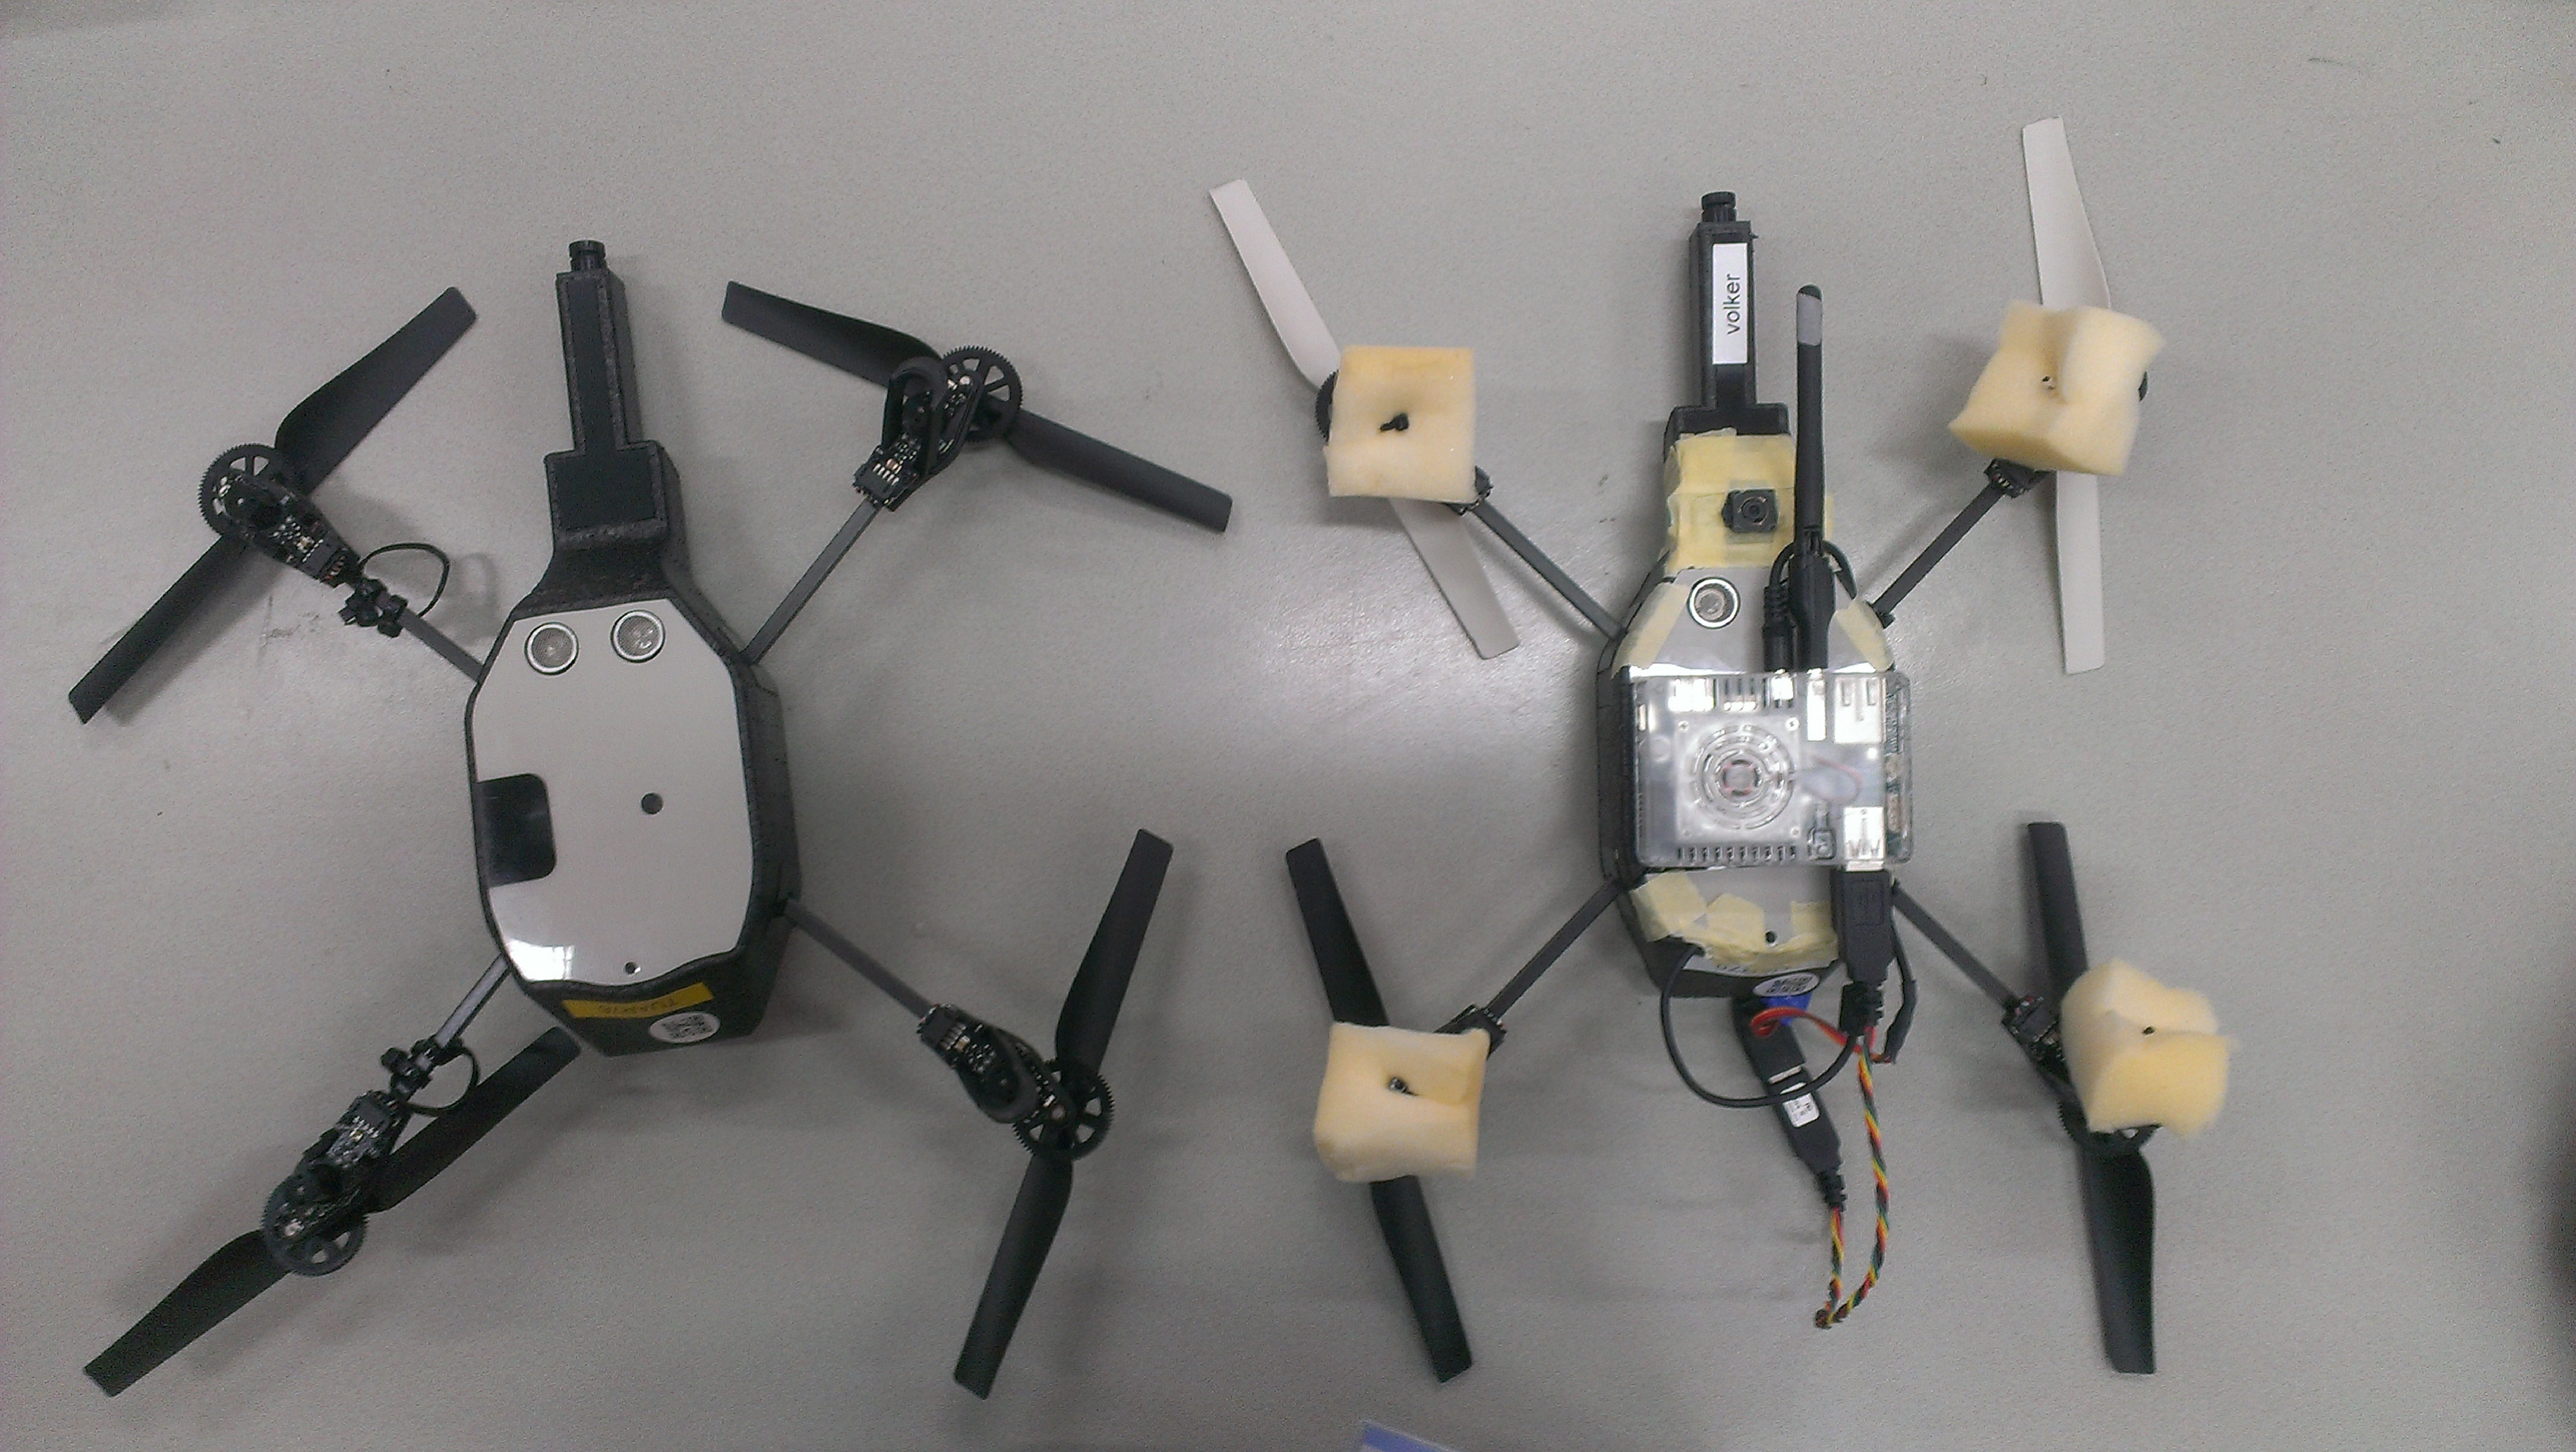
\includegraphics[width=0.7\columnwidth]{figures/comparison}
\caption{{\label{fig:comparison} Comparison of an unmodified Parrot AR.Drone.2.0 (left) and a
    modified version (right). The modified one was equipped with an
    Odroid XU-4 single board computer, a Logitech C525 HD camera, a
    WiFi module, and a USB connection between the Odroid board and the
    AR.Drone.2.0 flight controller.%
}}
\end{center}
\end{figure}

The Odroid processor has a full operating system (Ubuntu 15.04) and
allows to run arbitrary Linux software. While this setup allowed to
test algorithms on the rather powerful Odroid processor, the
additional weight resulted in unstable flight performance. Therefore,
we decided to modify the system to run it directly on-board of the UAV
and not on an external board such as the Odroid processor. This
removed the need for additional payload and made flight performance
very stable. Also, it reduced the need to buy and attach an external
processor and a point of failure. Another advantages is that the
framework can be easily ported to any UAV supported by the paparazzi
software. The disadvantages are that the on-board processors of many
MAVs have a lower performance than the Odroid processor. Additionally,
it required us to port the software from the high-level language
Python to the low-level language C without being able to rely on many
existing software libraries.

We decided to use the quadcopter \emph{Parrot Bebop Drone}
as prototype for all our tests. This UAV allow for navigating in
arbitrary directions without changing its yaw angle. Additionally,
several models show stable flight behavior, resulting in noise-free
images. It is equipped with a that allows for approximately 11 minutes
flying time. The UAV's dimensions are $28 \times 32 \times 3.6$\,cm
and it weighs 400\,g.

The UAV is equipped with two cameras: a front camera and a
downward-looking bottom camera. The proposed approach makes use of the
bottom camera only. This camera has a resolution of $640 \times 480$
pixels with a frequency of 30 frames per second. The UAV's processor
is a Parrot P7 dual-core CPU Cortex A9 with a tact rate of
800\,Mhz. It is equipped with 8~GB of flash memory. It runs a Linux
operating system. The full specifications of the UAV can be found at
\url{http://www.parrot.com/products/bebop-drone/}.

The original Bebop SDK was replaced with Paparazzi. Paparazzi is an
``open-source drone hardware and software project encompassing
autopilot systems and ground station software''. Its modular approach
allows for combining functions regarding stabilization, localization,
and control of UAVs.
The proposed approach is implemented as module in Paparazzi's computer
vision framework. Since low-level routines like accessing camera
information or attitude control for different platforms are already
implemented in Paparazzi, the proposed module can be readily used
across different platforms. Modules are written in the C programming
language and are cross-compiled on the host PC to make them suitable
for the UAV's processor. Afterwards, they are uploaded to the
microprocessor of the UAV, allowing for autonomous execution of the
compiled software. A downlink connection---from the UAV to the
groundstation---allows for monitoring the state of the aircraft (e.g.,
speed, altitude, position, battery status).

While the goal of the proposed system is to achieve an autonomous
system, monitoring the system is important for evaluation and safety
considerations. Figure~\ref{fig:gcs} shows the default ground control
station of Paparazzi.
For collecting data, real-time visualization of the position estimates
and enabling future users to keep track of the system states, a
graphical user interface (GUI) has been developed in the scope of this
thesis. The GUI is displayed in Figure~\ref{fig:gui}.

\begin{figure}[h!]
\begin{center}
\includegraphics[width=0.7\columnwidth]{figures/gui/default_figure}
\caption{{\label{fig:gui} Screenshot of the GUI. It displays
    the position esimate of the proposes framework, the ground truth
    position based on OptiTrack, the texton histogram, the Euclidean
    distances between OptiTrack and the system, and the uncertainty of
    the system (based on the spread of particles).%
}}
\end{center}
\end{figure}

The GUI displays the position estimate of the proposed framework, the
ground truth position based on OptiTrack, the texton histogram, the
Euclidean distances between OptiTrack and the system, the uncertainty
of the system, and the correlation between the uncertainty and the
Euclidean distance between the Optitrack and treXton estimates. The
GUI can be accessed using the \emph{Tool} menu in paparazzi.


\section{Pillar I: Training Set Generation}
\label{sec:mapping}

A main idea of the proposed method is to shift computational effort to
an offline phase, before the MAV is used on a repetitive task. This
shift is accomplished by using a light-weight machine learning
approach instead of a computationally more complex algorithm, such as
homography finding based on salient image keypoints.

Supervised machine learning needs a training set to find a mapping
from features to target values. In a computer vision-task, the
features represent image characteristics, such as average pixel values
or the amount of oriented gradients.

The proposed method is based on
histograms of textons. To create the training set, a convenient way is
to align image features---that is, the texton histograms---with
high-precision position estimates from a motion tracking system. 
These
systems can track rigid bodies at a high frequency within an error of
few millimeters. This allows to create high-quality training data
sets, where even low quality images can be mapped to the corresponding
$x,y$-position. 

This is achieved by saving the texton histogram on the MAV’s hard disk. The corresponding position from the motion tracking system is broadcast to the UAV via the ground station. The ground station receives the positions from the motion tracking system. 
The major disadvantages of the approach are that
motion tracking systems are usually expensive and time-consuming to
move to different environments.

As an alternative, we sought a low-budget and more flexible
solution. While the homography-based approach (Section xxx) shows high matching quality
for non-blurry images, it suffers from lacking robustness to noise
and the high processing time requirements. To exploit the advantages,
and straighten out the disadvantages, we used the approach in a preprocessing
step to obtain labeled training data of a known environment. This
allows to shift computational effort from the flight phase to a
pre-flight phase---paving the way for autonomous flights of MAVs with
limited processing power. It is based on two associated cornerstones
that are performed in an offline phase: the creation of an
\emph{orthomap} and finding a homography. The required image dataset
for both cornerstones can be obtained by using in-flight pictures of a
manual flight or by taking pictures with a hand-held camera.

For creating the orthomap, the images from the dataset have to be stichted
together to get a hyperspatial image of the scene. By orthorectifying
these pictures, different camera angles can be straightened out,
yielding seamless stitches. This results in a map of the
environment. The stitched image has a higher resolution than the
single images and contains a greater range of detail. The stitching
step includes challenges: a subset of the recorded images might be
distorted and each image must be orthorectified, otherwise perspective
transformations could hinder the stitching process. The images can be
orthorectified by estimating the most probable viewing angle based on
the set of all images. Since a downward-looking camera is attached to
the UAV, most images will be roughly aligned with the z-axis, given
slow flight.

For both steps, the software Agisoft
PhotoScan~\cite{agisoft2013agisoft} was used. The stitching process
can be time-consuming and error-prone. In some environments, an image
from a top view point can be taken capturing the entire area with
high-resolution camera, circumventing the need for stitching together
multiple images. Yet another method starts with an existing image and
modifies the environment accordingly---for example by painting the
floor or printing posters--to correspond to the image. In all cases,
we will describe the environment as \emph{map image}. 

Keypoints of the current image and the map image are detected and
described using the SIFT algorithm. This is followed by a matching
process, that identifies corresponding keypoints between both
images. These matches allow for finding a homography between both
images. For determining the $x, y$-position of the current image, the
center of it is projected on the reference image using the homography
matrix. The pixel position of the center in the reference image can be
used to determine the real world position by transforming the pixel
coordinates to real-world coordinates, based on the scale factors
$C_x$ and $C_y$, with $C_x = width(R) / width(I)$ and
$C_y = height(R) / height(I)$, where $W$ is the real-world
representation and $I$ the digital pixel image. This yields a dataset
of images, labeled with $x, y$ coordinates and the number of
matches. This process already introduces noise into the dataset, since
SIFT can have wrong and inaccurate matches.

\begin{figure}[h!]
\begin{center}
\includegraphics[width=0.7\columnwidth]{figures/map/default_figure}
\caption{{\label{fig:orthomap} This figure shows
    the created orthomap of a rather texture-rich floor. It is
    stitched together out of over 100 single images and represents a
    real world area of approximately $10\times10$ meters. Image
    distortions, non-mapped areas, and slightly skewed seams at
    several points are visible.%
}}
\end{center}
\end{figure}

\begin{figure}[h!]
\begin{center}
\includegraphics[width=0.7\columnwidth]{figures/sift/default_figure}
\caption{{\label{fig:homography} The
    image shows connected keypoint matches between the reference image
    on the left and the query image on the right. The green lines
    connect corresponding keypoints.%
}}
\end{center}
\end{figure}

In all cases, the result will be a labeled dataset of images and corresponding $x,y$-positions. The $x,y$-positions are of different quality depending on the used technique: orthomap-based, poster-based, or motion tracking-based. 


\section{Pillar II: Texton-based Approach}
\label{sec:textons}

In this section, the core of the proposed algorithm, the
implementation of the proposed texton framework is described.  The
histograms of textons are used as features for the $k$-Nearest
Neighbors ($k$NN) algorithm. The outputs of this regression technique
are possible $x,y$-coordinates for a given image.

In the following pseudo code, $M$ represents the number of particles,
$z_t^x$ the output of the texton framework at time $t$, and $f_t^x$
the estimated flow at time $t$.


Importantly, for generating the training dataset, no subsampling was
used. Therefore, the training dataset will not show any variance, if
the same images were used.

\subsection{Texton Dictionary Generation}
\label{sec:text-dict-gener}

For generating a suitable dictionary for a given environment, an
initial flight was performed. During this flight, 1000 randomly
selected image patches of size $w \times h = 6 \times 6$ were
extracted per image. In total, 100 images were used, resulting in
$100,000$ image patches, which were clustered to create a texton
dictionary. The resulting cluster centers---the prototypes of the
clustering result---are the textons~\cite{varma2003texture}. An
example of a learned dictionary can be found in
Figure~\ref{fig:dictionary}.

Different situations require different textons and a different number
of them. The choice of these parameters is map-dependent, and we set
it to 20 textons for all maps.


% TODO: Write some stuff about the low-level implementation

\subsection{$k$-Nearest Neighbors ($k$NN) algorithm}

% TODO: Write that one could also use a more efficient data structure than simply a list

For a given sample, the $k$-Nearest Neighbors ($k$NN) algorithm measures the similarity of this sample with all samples in the training dataset and outputs the $k$ most similar training examples. The similarity measure is a function that takes two samples as input and outputs a real value. We used the cosine similarity as similarity function, since it is bounded between 0 and 1. While other similarity measurements exists, the basic similarity measures—such as Euclidean distance—do not have a large impact on the results (Figure xxx). The choice of $k$ was based on the heuristic that XXX (TODO: write something like the sqrt of N or whatever) and on cross-validation.  
While the $k$NN algorithm is one of the simplest machine learning algorithms, it
offers several advantages: it is non-parametric, allowing for the
modeling of arbitrary distributions. Its capability to output multiple
predictions with an associated confidence allows for neat integration
with the proposed particle filter. Its simplicity comes together with transparency: it allows for spotting the possible sources of error: for example, wrongly labeled training examples. While the naive approach in using $k$NN for regression calculates the mean of the $k$ outputs, we decided to use a more complex method. This motivation is visualized in Figure XXX: If $k=2$ and the output values are distant to each other, averaging them would yield a value in the middle, which is with high certainty not the correct position. Over time, however, the ambiguity, can be resolved, when both estimates of the $k$NN model fall together. Compared to the Kalman filter, which is displayed in Figure XXX, the full Bayesian filter can immediately find the correct position. Since a full Bayesian filter is computationally complex, a variant that is based on Monte Carlo sampling was used: the particle filter. A more detailed description of the filtering technique can be found in the next section.  

% TODO: Compare particle filter with Kalman filter!!   

It often outperforms more sophisticated algorithms. A frequent critique regarding the $k$NN is its increasing computational complexity with an increasing size of the training dataset. However, its time complexity can be reduced by storing the training examples in an efficient manner, such as a binary tree structure. However, all of our training datasets were below 1000 images, resulting in fast predictions based on a list structure. 


\begin{algorithm}
\caption{{Particle filter update}}
\label{alg:particle_filter}
\begin{algorithmic}[1]
  \Procedure{Particle\_Filter}{$\mathcal{X}_{t-1}, z_t^x, z_t^y, f_t^x, f_t^y$}
  % q is process noise, r is measurement noise
  \State $q_x^2 = 15$, $q_y^2 = 15$, $r_x^2 = 100$, $r_y^2 = 100$
  \LineComment{Particle update}
  \For{$m = 1$ to $M$}
  \State sample $x_t^{[m]} \sim \mathcal{N}(x_{t-1}^{[m]} + f_t^x, q_x^2)$
  \State sample $y_t^{[m]} \sim \mathcal{N}(y_{t-1}^{[m]} + f_t^y, q_y^2)$
  \State $w_t^{[m]} \gets p(z_t^x \mid x_t^{[m]}) p(z_t^y \mid y_t^{[m]})$
  % Resampling wheel
  \EndFor
  \LineComment{Importance resampling}
  \State $\mathcal{X}_t \gets$ \Call{Resampling\_Wheel}{$\mathcal{X}_{temp}, w_t$}
  \EndProcedure
\end{algorithmic}
\end{algorithm}

\begin{algorithm}
\caption{{Resampling wheel}}
\label{alg:resampling_wheel}
  \begin{algorithmic}[1]
    \Procedure{Resampling\_Wheel}{$\mathcal{X}_{temp}, w_t$}
    \State $\mathcal{X}_t \gets \emptyset$
    \State sample $idx \sim M\cdot\mathcal{U}(0, 1)$
    \State $\beta \gets 0$
    \State $mw = max(w_t)$
    \For{$m = 1$ to $M$}
    \State $\beta \gets \beta + \mathcal{U}(0, 1)\cdot 2\cdot mw$
    \While{$\beta > w_t[idx]$}
    \State $\beta \gets beta - w_t[idx]$
    \State $idx \gets (idx + 1) \mod M$
    \EndWhile
    \State add $\mathcal{X}_{temp}[idx]$ to $\mathcal{X}_t$
    \EndFor
\EndProcedure
  \end{algorithmic}
\end{algorithm}

\begin{algorithm}
\caption{{Initialize texton framework}}
\label{alg:trexton_init}
  \begin{algorithmic}[1]
    \Procedure{Init\_TreXton}{}
    \State $t \gets 0$ 
    %\State textons $\gets$ \Call{csv\_read\_textons}{}
    %\State ann $\gets$ \Call{load\_neural\_network}{}
    \State $\mathcal{X}_0 \gets$ \Call{init\_particles}{}
    \EndProcedure
  \end{algorithmic}
\end{algorithm}

\begin{algorithm}
\caption{{Run texton framework}}
\label{alg:trexton_run}
  \begin{algorithmic}[1]
    \Procedure{Run\_TreXton}{}
    \State $t \gets t+1$ 
    \State $I_t \gets$ \Call{Receive\_Img\_from\_Webcam}{}
    \State $\widetilde{I_t} \gets$ \Call{Standardize\_Image}{$I_t$}
    \State $\mathcal{H}_t \gets$ \Call{Get\_Histogram}{$\widetilde{I_t}$}
    \State $z_t^x, z_t^y \gets$ \Call{Predict\_Position}{$\mathcal{H}_t$}
    \State $f_t^x, f_t^y \gets$ \Call{Calc\_Flow}{$I_t$}
    \State $\mathcal{X}_t \gets$
    \Call{Particle\_Filter}{$\mathcal{X}_{t-1}, z_t^x, z_t^y, f_t^x,
      f_t^y$}
    \State $x_t, y_t \gets$ \Call{Weighted\_Average}{$\mathcal{X}_t$}
    \State \Call{Send\_Pos}{$x_t, y_t$}
    \EndProcedure
  \end{algorithmic}
\end{algorithm}


\section{Filtering and Smoothing}
\label{sec:filtering}


Computer vision-based estimations are usually noisy or ambiguous, and
so is the proposed system: beginning with the estimations of the
homographies, the ground truth is already based on possibly faulty
labelings. Texton histograms obtained during flight will not perfectly
match the ones in the training data set: blur, lighting settings,
viewing angles and other variables change the shape of the texton
histograms.

To filter out outliers and smooth the estimations, a popular filter
choice is the Kalman filter. However, the Kalman filter is not able to
represent multimodal probability distributions. This makes it rather
unsuitable for the presented approach: if the $k$nn model outputs two
predictions, one would need to use average of these predictions and
feed this value to the Kalman Filter. This approach can lead to biased
predictions, especially, if the the model outputs belong to distant
locations--- to similar texton distributions at these positions.

Instead, the more powerful general Bayesian filter could simultaneously keep
account of both possible locations and resolve the ambiguity as soon
as one location can be favored. In this case, the predictions of the
$k$ neighbors are directly fed into the particle filter without
averaging them first. The filter is able to smooth the estimations,
handle uncertainty, and simultaneously keep track of several competing
position estimations. Since the calculation of a full Bayesian filter is computationally intractable, a particle filter which is based on sampling was used as approximation. 

In general, particle filters estimate the posterior probability of the
state given observations. Specifically, this means that finding the
position of the UAV can be described as $p(X_t \mid Z_t)$, where $X_t$
is the state vector at time $t$ ($x,y$-position, heading, speed,
acceleration) and $Z_t$ are the measurements ($z_1, ..., z_t$, where
each $z_i$ represents the $x,y$ output of the proposed algorithm) up
to time $t$. The state vector is \emph{hidden}, since the variables
cannot be measured directly, therefore the situation can be described
using a hidden Markov model. Instead, noisy or ambiguous data can be
obtained through the proposed algorithm.

The weighted particles are a discrete approximation of the posterior
probability function ($pdf$) of the state vector.

Particle filters have several advantages. First, one can represent
uncertainty by the variance of the state variables of the
particles. Second, the particle filter allows for \emph{sensor fusion}, and
can integrate IMU data or optical flow into the position estimation.
A major disadvantage is the rather high computational complexity. This
can be circumvented by reducing the amount of particles (trading off
speed and accuracy)---allowing for adapting the computational payload
to the used processor.

The used particle filter is initialized using 100 particles at random
$x, y$-positions. To incorporate the distances, the sensor model $p(z
\midx) = \frac{p(x \mid z)p(z)}{p(x)}$ is used, where $\textbf{x} =
((x_1, y_1), (x_2, y_2), \ldots, (x_k, y_k))^T$. A two-dimensional
Gaussian model was used for each point. The parameters of the Gaussian
have been determined by comparing of the positions based on the motion
tracking system with the predictions of the proposed system. This
results in values for the variances in $x$ and $y$, the correlation
$\rho$ between $x$ and $y$. The mean values $\mu$ were set to zero
(no-systematic bias). Figure~\ref{fig:measurementmodel} shows the
results of one such evaluation.

\begin{figure}[h!]
\begin{center}
\includegraphics[width=0.7\columnwidth]{figures/measurement_model/default_figure}
\caption{{\label{fig:measurementmodel} Measurement model showing the delta x and delta y
    positions%
}}
\end{center}
\end{figure}

This allows to make use of the information in all $k$ neighbors and
keep track of a multimodal distribution. While keeping track of a
multimodal distribution allows for incorporating several possible
states of the system, the problem arises of which mode is the best
one. Using a weighted average of the modes would again introduce the
problem, that the weighted average falls into a low density
region. Therefore, the maximum a posteriori estimate, as described in
\cite{driessen2008map} is used. This approach uses the following
formula to obtain the MAP estimate:

Therefore, the final position estimate is equal to the position of one
of the particles.

\begin{align}
  s_k^{MAP}  &= \argmax_{s_k}{p(s_k \mid Z_k)}\\
             &= \argmax_{s_k}{p(z_k \mid s_k) p(s_k \mid Z_{k-1})} 
\end{align}

Therefore, the MAP estimator in our case is

\begin{align}
s_k^{MAP} = \argmax_{s_k} \lambda^M(s_k)
\end{align}
with

\begin{align}
\lambda^M(s_k) = p(z_k \mid s_k) \sum_{j=1}^Mp(s_k \mid s_{k-1}^j)w^j_{k-1}
\end{align}

This function is now only evaluated at a finite, chosen number of
states, the particles, using

\begin{align}
\hat{s}_k^{MAP} = \argmax_{s_k \in \{s_k^i \mid i=1,\ldots,N\}} \lambda^M(s_k)
\end{align}

In this formula, $p(z_k \mid s_k)$ is the likelihood of the particle
$s_k$ given the current measurement $z_k$. In our setting, this
probability is equal to the weight of the particle $z_k$, therefore
$p(z_k \mid s_k) = w^i_k$.

The estimation of \emph{uncertainty} is a core part of the proposed
approach, being important for safety and accuracy. Therefore,
uncertainty was modeled using the spread of the particles.

In every time step, the particles of the filter get updated based on
the optical flow estimates. These estimates are noisy, as illustrated
in Figure~\ref{fig:edgeflow}. Additionally, optical flow estimates
aggregate noise over time, since each estimate is dependent on the
previous one, leading to drift (\emph{relative position
  estimates}). In contrast, the machine learning-based method makes
independent predictions. While this allow for avoiding accumulating
errors, the predictions do not dependent on each other, and might be
`jumping' between two points. To combine the advantages of both
methods, and leverage out the disadvantages, the particle filter is
used.

An idea was to include the similarity to the neighbors as confidence
value, thus reducing the measurement noise, if a high similarity
between current histogram and a training histogram is
achieved. However, we found no correlation between these
variables. Figure~\ref{fig:cor_sim_measurement} displays the
dependence structure.

\begin{figure}[h!]
\begin{center}
\includegraphics[width=0.7\columnwidth]{figures/fig_cor_sim_confi/default_figure}
\caption{{\label{fig:cor_sim_confi} Dependence structure between similarity of histograms and
    measurement error.%
}}
\end{center}
\end{figure}

Another idea---if the homography-based approach is used for
labeling---was to use the amount of detected keypoints as confidence
value. However, again, no linear relation between the two variables
could be found (Figure~\ref{fig:cor_sift_confi}).

\begin{figure}[h!]
\begin{center}
\includegraphics[width=0.7\columnwidth]{figures/fig_cor_sift_confi/default_figure}
\caption{{\label{fig:cor_sift_confi} Dependence structure between number of keypoints and quality
    of the measurement.%
}}
\end{center}
\end{figure}

